
%%% - intro
\begin{frame}
\frametitle{Key ideas for fast computation}
Uncertainty quantification (UQ) typically requires a high number of simulations using basic linear algebra operations. Then two things come in handy :

  \begin{itemize}
    \item fast linear algebra decomposition ($QR$, $LL^T$, ...)
    \item efficient data strucutures
  \end{itemize}

If many simulations are 'similar' there is most likely a low-rank property somewhere to be exploited. Low-rank property in linear algebra leads to fast computations AND efficient structures!

We shall present two efficient methods :
  \begin{itemize}
    \item random linear algebra for medium-sized problems (on a simple example!)
    \item the $\mathcal{H}$-matrix framework (much more detailed)
  \end{itemize}
\end{frame}


%%% - intro: model problem
\begin{frame}
\frametitle{Model problem}
Suppose we are interested in eigenvalues (and/or eigenvectors) of a covariance matrix of the form $C_X = X^TX$ where X is of size $m \times n$.
Several methods:
  \begin{itemize}
    \item eigenvalue decomposition of $C_X$: $\mathcal{O}(n^3)$ operations and conditionning of normal equations is bad!
    \item SVD decomposition of X: (better, still expensive) $\mathcal{O}(mn^2)$ operations
    \item \alert{what else?}
  \end{itemize}
\end{frame}

%%% - random QR
\begin{frame}
\frametitle{Randomness and linear algebra}
\textbf{Basic idea:} using random test matrix $\Omega$ and the fact that any orthogonal basis of $\mathrm{ran}(Y)$ with $Y=A \Omega$ is a good approximate basis for $\mathrm{ran}(A)$. $Y$ has a less columns than $A$ so $QR$ is cheaper! 

  \begin{algorithm}[H]
  \caption{A simple random QR decomposition}
  \label{rQR}
  \begin{algorithmic}[1]

  \REQUIRE A matrix $\mathbf{A}$ of size $m \times n$, an oversampling parameter $l$.
  \ENSURE An orthogonal basis $\mathbf{Q_Y}$ of $\mathrm{ran}(\mathbf{A})$. 

  \STATE Draw a random matrix $\mathbf{W}$ of size $n \times l$.
  \STATE Form product $\mathbf{Y}$ : $\mathbf{Y} = \mathbf{A} \mathbf{W}$. 
  \STATE Form the $QR$ decomposition of the matrix $\mathbf{Y}$ : $\mathbf{Y}=\mathbf{Q_Y} \mathbf{R}$.
  \RETURN
  \end{algorithmic}
  \end{algorithm}
\end{frame}


%%% - random SVD
\begin{frame}
\frametitle{A random SVD}
  \begin{algorithm}[H]
  \caption{A simple random SVD decomposition}
  \label{rSVD}
  \begin{algorithmic}[2]
  \REQUIRE A matrix $\mathbf{A}$ of size $m \times n$, an orthogonal matrix $\mathbf{Q}$ tq $\mathbf{A} \simeq \mathbf{Q}\mathbf{R}$.
  \ENSURE An approximate $SVD$ decomposition of $\mathbf{A}$, $\mathbf{A} \simeq \mathbf{U} \mathbf{\Sigma} \mathbf{V}^T$.

  \STATE Construct the projection matrix $\mathbf{B}=\mathbf{Q}^T \mathbf{A}$.
  \STATE Form the SVD of $\mathbf{B}$ : $\mathbf{B} = \mathbf{\tilde{U}} \mathbf{\Sigma} \mathbf{V}^T$. 
  \STATE Build the matrix $\mathbf{U} = \mathbf{Q} \mathbf{\tilde{U}}$.

  \RETURN
  \end{algorithmic}
  \end{algorithm}
\end{frame}


%%% - a numerical example
\begin{frame}
\frametitle{A numerical example}

Say $X \in \mathbb{R}^{m \times n}$ is a discrete approximate of a random process $X(t,\omega)$ over $[-1,1]$ with exponential covariance function $C(s,t) = e^{-|t-s|}$. We are still interested in eigenvalues of $C_X$. In that case, we can prove that $\lambda_n / \lambda_1 = \mathcal{O}(n^{-2})$.

In the following example we choose $m=6400$ and $n=1000$.
\end{frame}

%%% - Eigenvalues profile
\begin{frame}
\frametitle{Eigenvalues estimates}

\begin{columns}[t]
  \begin{column}{5cm}
\begin{figure}[H]
\begin{center}
  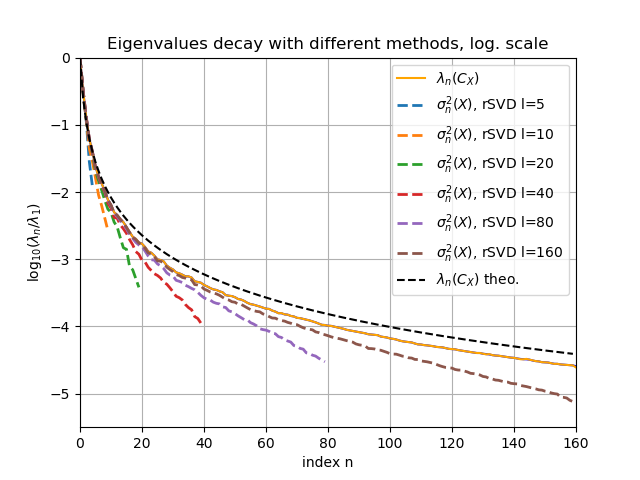
\includegraphics[scale=0.3]{./img/eigenValues_1.png}
  \caption{Eigenvalues decay.}
\end{center}
\end{figure}

\end{column}
  
  \begin{column}{5cm}
    \begin{figure}[H]
    \begin{center}
  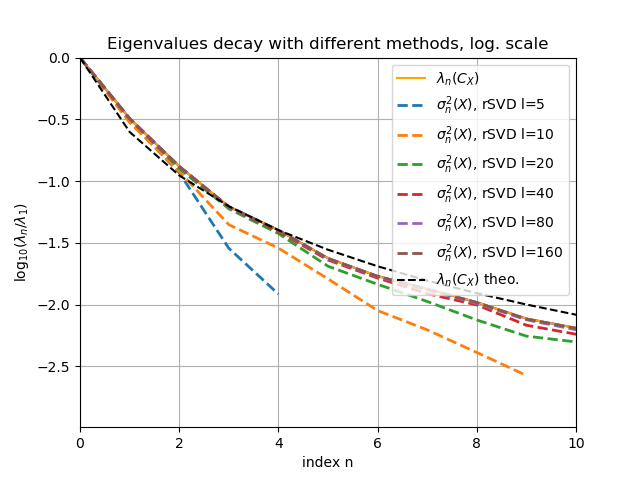
\includegraphics[scale=0.3]{./img/zoom-1.png}
  \caption{Eigenvalues decay - the first 10.}
     \end{center}
     \end{figure}

  \end{column}
 \end{columns}  
\end{frame}

%%% - Timings
\begin{frame}
\frametitle{Case summary}
\begin{table}[H]
\centering
\begin{tabular}{rrrr}
\hline
test matrix \# cols.  & elapsed time (s) &   $\sum \lambda_n$ & rel. error \\
\hline
               5 & 0.021            & 4950345.8          & 0.253      \\ 
              10 & 0.027            & 5894250.4          & 0.111      \\ 
              20 & 0.038            & 6309314.4          & 0.048      \\
              40 & 0.060            & 6478969.3          & 0.023      \\
              80 & 0.068            & 6556588.8          & 0.011      \\ 
             160 & 0.131            & 6598333.6          & 0.005      \\
\hline
\end{tabular}
\caption{Example summary for random SVD \label{tab:rSVD}}                
\end{table}

\begin{itemize}
  \item For reference : $\mathrm{trace}(C_X) = 6632269.0$
  \item elapsed time for full SVD: 0.663s
  \item elapsed time for \textit{numpy.linalg.eigs}: 107.307.
\end{itemize}
\end{frame}

%%% - Partial conclusion
\begin{frame}
\frametitle{Partial conclusion}
\begin{itemize}
  \item many articles in the literature,
  \item random SVD is implemented in OPENTURNS,
  \item generally behave better than classical methods,
  \item \alert{what if the problem is larger ?}
\end{itemize}
\end{frame}
